A detailed and clear contextualization of the problem is presented below, specifying the area in which it is framed—namely, digital communication and social media—and highlighting its relevance. The main objective is to analyze and mitigate the presence of hate speech on social media platforms through machine learning techniques.

Over the past couple of decades, with the advancement of technology and the internet, social media platforms have become increasingly relevant. These platforms have enabled the easier dissemination of information, its democratization, and global connectivity.

In 2024, this growth continued. Facebook led in the number of monthly active users, reaching over 3 billion—something no other platform has achieved to date. YouTube followed with 2.5 billion users, while Instagram and WhatsApp occupied third place, each with around 2 billion users. As a result, social media platforms also generate substantial revenue; for example, Facebook alone generates more than 80 billion USD annually. These figures clearly show the significance of social media platforms, both in terms of user base and economic impact.

However, social media has also introduced new challenges. With the ability to post content at any time and on nearly any topic, hate speech directed at individuals or groups has become increasingly prevalent. This type of speech has begun to impact society. In January 2023, attacks were carried out on Brazilian government buildings, and on January 6, 2021, the United States Capitol was stormed. Both incidents occurred after certain groups spread dangerous rhetoric and false claims against others.

A deeper analysis of this issue on platforms such as Facebook and Instagram reveals the following figures:

\begin{figure}[htbp]
    \centering
    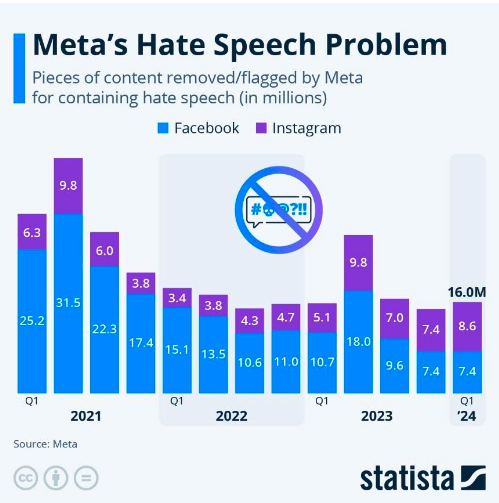
\includegraphics[width=0.9\linewidth]{images/MetaHateSpeechProblem.png}
    \caption{Meta's hate speech problem. Source: \cite{zandt2024}.}
    \label{fig:meta_hate_speech_problem}
\end{figure}
 
As observed, millions of pieces of content are removed every year due to the presence of hate speech in various forms.

Additionally, on the platform X (formerly Twitter), there has been a notable increase in such comments. Hate speech has generally risen by 50\%, while transphobic, homophobic, and racist comments have increased by 260\%, 30\%, and 42\%, respectively.

This highlights the significant relevance of hate speech in the social context, particularly on social media. Effectively identifying and removing such comments is a fundamental task that social platforms must undertake.

Therefore, the goal of this project is to develop \textit{Machine Learning} and \textit{Deep Learning} models to effectively classify comments in English, since this is one of the most commonly used languages. For instance, 55\% of tweets on X are published in English.

The aim is to compare the implemented models and determine which one delivers the best results.
